% =====================================================================
%  Case study: Amazon.com on both factor panels
%
%  Build:  python -m scripts.build_case_study --pdf
%  (the figures and every number in the prose are generated first)
% =====================================================================
\documentclass[11pt,a4paper]{article}

\usepackage[T1]{fontenc}
\usepackage[utf8]{inputenc}
\usepackage[english]{babel}
\usepackage{mathpazo}
\usepackage[scaled=0.90]{helvet}
\usepackage{microtype}

\usepackage[a4paper,top=26mm,bottom=24mm,left=26mm,right=26mm]{geometry}
\usepackage{amsmath,amssymb}
\usepackage{booktabs,array,tabularx}
\usepackage{graphicx}
\usepackage{xcolor}
\usepackage{titlesec}
\usepackage{fancyhdr}
\usepackage[font=small,labelfont=bf,labelsep=period]{caption}
\usepackage{enumitem}
\usepackage[hidelinks]{hyperref}

\definecolor{navy}{HTML}{23456B}
\definecolor{ink}{HTML}{1A1A1A}
\definecolor{rule}{HTML}{C9C4BA}
\definecolor{paper}{HTML}{F7F5F0}
\definecolor{brick}{HTML}{8C3A2E}
\definecolor{moss}{HTML}{4A6B4A}

\hypersetup{
  colorlinks=true, linkcolor=navy, urlcolor=navy,
  pdftitle={Amazon.com on both factor panels},
  pdfauthor={Bastian Offermann},
}

\titleformat{\section}
  {\normalfont\sffamily\large\bfseries\color{navy}}{\thesection}{0.8em}{}
\titleformat{\subsection}
  {\normalfont\sffamily\normalsize\bfseries\color{ink}}{\thesubsection}{0.7em}{}
\titlespacing*{\section}{0pt}{2.4ex plus 1ex minus .2ex}{1.1ex plus .2ex}

\pagestyle{fancy}
\fancyhf{}
\renewcommand{\headrulewidth}{0.3pt}
\renewcommand{\headrule}{\hbox to\headwidth{\color{rule}%
  \leaders\hrule height \headrulewidth\hfill}}
\fancyhead[L]{\footnotesize\sffamily\color{navy}Case study · Amazon.com on both factor panels}
\fancyhead[R]{\footnotesize\sffamily\color{navy}\thepage}

\setlength{\parskip}{0.6ex}
\setlength{\parindent}{0pt}
\renewcommand{\arraystretch}{1.18}

\newcommand{\code}[1]{\texttt{\small #1}}
\newcommand{\orth}{\textcolor{navy}{\textbf{orthogonalised}}}
\newcommand{\rawp}{\textcolor{brick}{\textbf{raw}}}

% A pull-quote: the one sentence a reader should take from the section.
\newsavebox{\takeawaybox}
\newenvironment{takeaway}
  {\par\vspace{1.4ex}%
   \begin{lrbox}{\takeawaybox}\begin{minipage}{\dimexpr\textwidth-2.2em\relax}%
   \vspace{0.9ex}\hspace{0.4em}\begin{minipage}{\dimexpr\textwidth-3.4em\relax}
   \small\sffamily\color{ink}}
  {\end{minipage}\vspace{0.9ex}%
   \end{minipage}\end{lrbox}%
   \noindent\colorbox{paper}{%
     \textcolor{navy}{\rule{2.2pt}{\dimexpr\ht\takeawaybox+\dp\takeawaybox\relax}}%
     \usebox{\takeawaybox}}\par\vspace{1.6ex}}

% Every figure quoted in the prose comes from here.
% Generated by scripts/build_case_study.py — do not edit by hand.
\newcommand{\amzFirst}{2000-01-04}
\newcommand{\amzLast}{2026-07-22}
\newcommand{\amzDays}{6,671}
\newcommand{\amzVol}{48.0\%}
\newcommand{\amzRet}{16.4\%}
\newcommand{\amzWorst}{-28.5\%}
\newcommand{\amzBest}{29.6\%}
\newcommand{\amzKurt}{13.1}
\newcommand{\winO}{260}
\newcommand{\adjRO}{0.420}
\newcommand{\condO}{54}
\newcommand{\condMaxO}{134}
\newcommand{\vifO}{25}
\newcommand{\vifMaxO}{90}
\newcommand{\shiftO}{5.6}
\newcommand{\corrO}{0.906}
\newcommand{\residO}{27.4\%}
\newcommand{\exclO}{0}
\newcommand{\nfcO}{248}
\newcommand{\biasO}{0.947}
\newcommand{\zstdO}{1.040}
\newcommand{\zkurtO}{13.4}
\newcommand{\mzbO}{0.643}
\newcommand{\mzpO}{0.249}
\newcommand{\mzrO}{0.089}
\newcommand{\exNFO}{200}
\newcommand{\exEFO}{260}
\newcommand{\exNNO}{81}
\newcommand{\exENO}{52}
\newcommand{\kupFO}{$<$0.001}
\newcommand{\kupNO}{$<$0.001}
\newcommand{\chrFO}{$<$0.001}
\newcommand{\sampleO}{2005-10-28}
\newcommand{\predLastO}{36.1\%}
\newcommand{\shareLastO}{68\%}
\newcommand{\betaEqGO}{1.46}
\newcommand{\vifOfEqGO}{11}
\newcommand{\betaEqUSO}{0.23}
\newcommand{\vifOfEqUSO}{8}
\newcommand{\betaMomO}{-0.62}
\newcommand{\vifOfMomO}{2}
\newcommand{\sdEqGO}{0.38}
\newcommand{\sdEqUSO}{1.09}
\newcommand{\loEqGO}{0.44}
\newcommand{\hiEqGO}{2.40}
\newcommand{\loEqUSO}{-2.69}
\newcommand{\hiEqUSO}{2.58}
\newcommand{\corrPairO}{-0.08}
\newcommand{\topBlockO}{Equity Market}
\newcommand{\topBlockShareO}{33\%}
\newcommand{\specShareO}{33\%}
\newcommand{\winR}{260}
\newcommand{\adjRR}{0.455}
\newcommand{\condR}{201}
\newcommand{\condMaxR}{2,579}
\newcommand{\vifR}{4,988}
\newcommand{\vifMaxR}{230,726}
\newcommand{\shiftR}{7.9}
\newcommand{\corrR}{0.885}
\newcommand{\residR}{26.5\%}
\newcommand{\exclR}{16}
\newcommand{\nfcR}{232}
\newcommand{\biasR}{0.907}
\newcommand{\zstdR}{0.992}
\newcommand{\zkurtR}{12.2}
\newcommand{\mzbR}{0.441}
\newcommand{\mzpR}{0.009}
\newcommand{\mzrR}{0.105}
\newcommand{\exNFR}{188}
\newcommand{\exEFR}{258}
\newcommand{\exNNR}{72}
\newcommand{\exENR}{52}
\newcommand{\kupFR}{$<$0.001}
\newcommand{\kupNR}{0.007}
\newcommand{\chrFR}{$<$0.001}
\newcommand{\sampleR}{2005-12-29}
\newcommand{\predLastR}{37.0\%}
\newcommand{\shareLastR}{66\%}
\newcommand{\betaEqGR}{1.93}
\newcommand{\vifOfEqGR}{169}
\newcommand{\betaEqUSR}{1.53}
\newcommand{\vifOfEqUSR}{73}
\newcommand{\betaMomR}{-0.60}
\newcommand{\vifOfMomR}{6}
\newcommand{\sdEqGR}{1.94}
\newcommand{\sdEqUSR}{1.70}
\newcommand{\loEqGR}{-2.12}
\newcommand{\hiEqGR}{7.18}
\newcommand{\loEqUSR}{-2.37}
\newcommand{\hiEqUSR}{6.25}
\newcommand{\corrPairR}{-0.37}
\newcommand{\topBlockR}{Equity Market}
\newcommand{\topBlockShareR}{38\%}
\newcommand{\specShareR}{35\%}
\newcommand{\shareMean}{53\%}
\newcommand{\shareMajority}{64\%}
\newcommand{\amzWindowEnd}{2026-07-22}
\newcommand{\orthSpec}{88b9b8e7d5af}
\newcommand{\rawSpec}{a8d1454d32ea}


\begin{document}

% ---------------------------------------------------------------- title
\thispagestyle{empty}
\vspace*{0.4cm}
{\raggedright
{\color{rule}\rule{\textwidth}{0.8pt}}\\[1.8ex]
{\sffamily\footnotesize\color{brick}\MakeUppercase{Case study}\par}
\vspace{0.8ex}
{\sffamily\LARGE\bfseries\color{navy} One security, two factor panels\par}
\vspace{1.0ex}
{\sffamily\large\color{ink} What the model says about Amazon.com --- and which
version of it you should believe\par}
\vspace{1.6ex}
{\color{rule}\rule{\textwidth}{0.8pt}}\\[1.8ex]
{\small Bastian Offermann \quad·\quad September 2026 \quad·\quad
 \code{US:AMZN} \quad·\quad \amzDays{} trading days\par}
}

\vspace{2.4ex}

\begin{takeaway}
\textbf{The short version.} Estimated on identical settings, the \rawp{} panel fits
Amazon better in sample --- adjusted $R^2$ of \adjRR{} against \adjRO{} --- and
forecasts its risk distinctly worse out of it. Its Mincer-Zarnowitz slope is
\mzbR{} against \mzbO{}, and where the orthogonalised forecast survives the joint
test ($p$ = \mzpO{}) the raw one does not ($p$ = \mzpR{}). It also throws away
\exclR{} windows as unusable, against \exclO{}. The orthogonalised panel is the one
to forecast with. The raw panel is the one to explain an exposure with, and this
document shows exactly where the two disagree.
\end{takeaway}

% =====================================================================
\section{The security}

Amazon is a deliberately awkward test case. Over \amzDays{} trading days from
\amzFirst{} it compounded at \amzRet{} a year at \amzVol{} annualised volatility,
with a worst day of \amzWorst{} and a best of \amzBest{}, and an excess kurtosis of
\amzKurt{}. It changed what it was twice --- online retailer, then cloud
infrastructure business --- without changing its ticker, which is precisely the
situation a return-based model is built for and a holdings-based one struggles
with.

\begin{figure}[htbp]
\centering
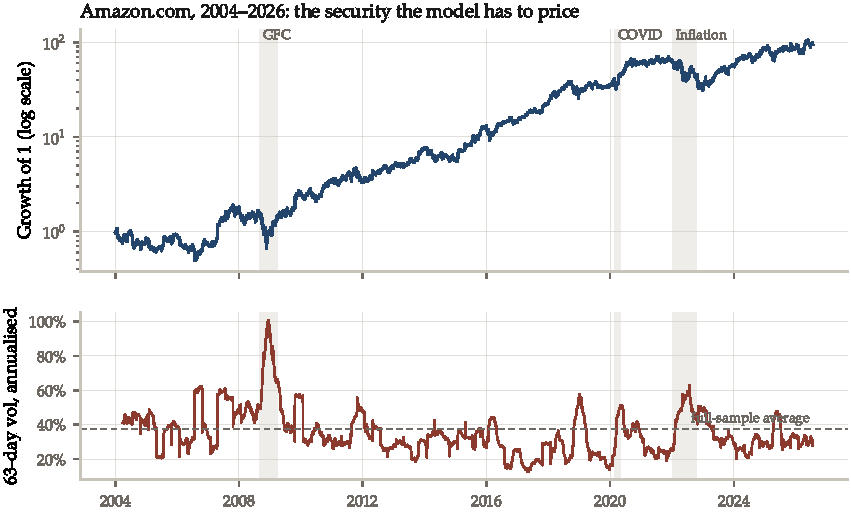
\includegraphics[width=\textwidth]{figures/amzn-security}
\caption{The security, before any model touches it. Shaded bands mark the global
financial crisis, the COVID drawdown and the 2022 inflation shock; they are
editorial context drawn on the chart, never an output of the model.}
\end{figure}

\subsection{The experiment}

Two specifications, identical in every parameter except the factor panel they read.

\begin{center}
\small
\begin{tabular}{@{}lll@{}}
\toprule
 & \textcolor{navy}{\textbf{Orthogonalised}} & \textcolor{brick}{\textbf{Raw}} \\
\midrule
Specification & \code{\orthSpec\ldots} & \code{\rawSpec\ldots} \\
Factor panel & block-hierarchy residuals & excess returns, before residualisation \\
Window / step & 252 days, rolled monthly & 252 days, rolled monthly \\
Estimator & OLS, Newey-West HAC & OLS, Newey-West HAC \\
Covariance & blend (EWMA + shrunk) & blend (EWMA + shrunk) \\
Forecast horizon & 21 days & 21 days \\
\addlinespace
Windows estimated & \winO{} & \winR{} \\
Forecasts scored & \nfcO{} & \nfcR{} \\
Sample & from \sampleO{} & from \sampleR{} \\
\bottomrule
\end{tabular}
\end{center}

Everything that follows is a difference between these two columns, and the only
thing that differs is which version of the same forty factors the regression sees.

% =====================================================================
\section{What the model says Amazon \emph{is}}

\begin{figure}[htbp]
\centering
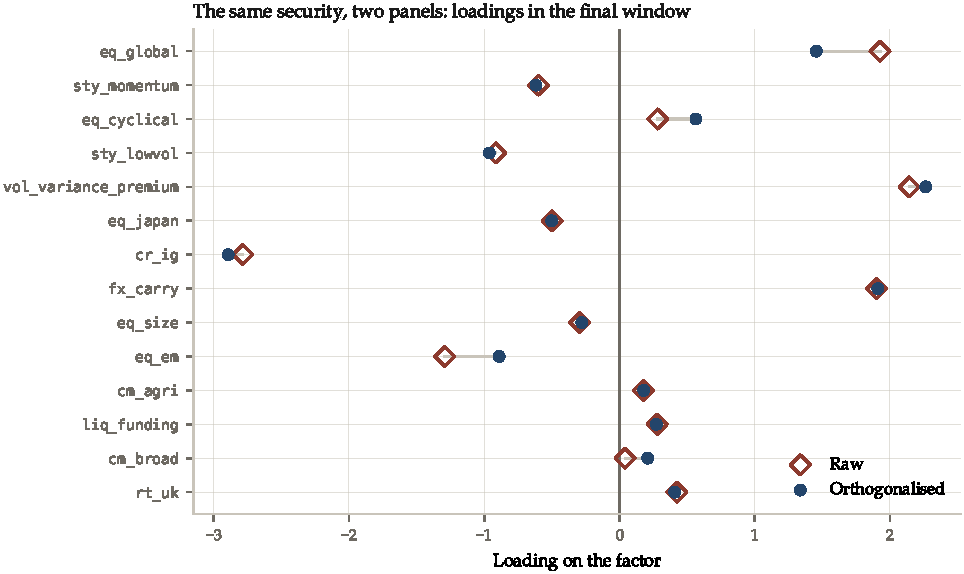
\includegraphics[width=\textwidth]{figures/amzn-loadings}
\caption{Loadings in the final window (\amzWindowEnd{}), the fourteen largest by
orthogonalised $t$-statistic. Where the two markers sit on top of one another the
panels agree; where they separate, the raw loading is absorbing something the
hierarchy has already assigned elsewhere.}
\end{figure}

Read the equity rows first, because that is where the panels are supposed to
disagree and where the disagreement is largest.

On the \orth{} panel, Amazon loads \betaEqGO{} on \code{eq\_global} and
\betaEqUSO{} on \code{eq\_us}. That is the honest reading of a hierarchy: global
equity carries the market exposure, and the US residual --- what US equity does
\emph{beyond} global equity --- adds almost nothing on top. One number does the
work.

On the \rawp{} panel the same security loads \betaEqGR{} on \code{eq\_global}
\emph{and} \betaEqUSR{} on \code{eq\_us}. Both are large, both are positive, and
they are describing the same exposure twice, because on the raw panel
\code{eq\_us} and \code{eq\_global} are near-copies of each other. The variance
inflation factors say so out loud: \vifOfEqGR{} and \vifOfEqUSR{} on the raw panel,
against \vifOfEqGO{} and \vifOfEqUSO{} on the orthogonalised one.

\begin{takeaway}
Neither reading is wrong, and they answer different questions. \emph{``How much
equity risk does Amazon carry?''} is the raw panel's question, and the answer is
the sum. \emph{``Which part of the equity complex explains Amazon?''} is the
orthogonalised panel's, and the answer is: global beta, plus a cyclical tilt, minus
momentum. Only the second can be decomposed without double-counting.
\end{takeaway}

The non-equity rows are more interesting than they look. \code{sty\_momentum} comes
out at \betaMomO{} on both panels --- a genuinely negative momentum loading, which
for a stock that has compounded at \amzRet{} a year is counter-intuitive until you
remember what the factor is: a long-only momentum fund residualised against market
and sector. Amazon is a large, widely held growth name, not a momentum name, and
the model is saying so consistently on both panels. Agreement across panels is
itself evidence: a loading that survives residualisation is not an artefact of the
design.

% =====================================================================
\section{Stability: the same exposure, month after month}

\begin{figure}[htbp]
\centering
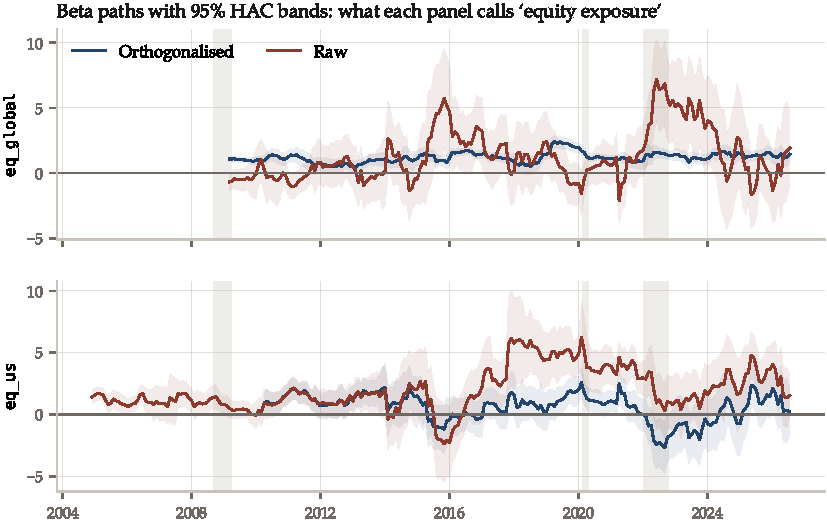
\includegraphics[width=\textwidth]{figures/amzn-beta-paths}
\caption{Equity beta through time with 95\% HAC bands. Top: global equity. Bottom:
US equity. The orthogonalised global-equity beta is the flat navy line in the upper
panel; everything else on the chart is the same exposure, estimated less stably.}
\end{figure}

Start with the top panel, which is the cleanest single picture in this document.
Amazon's loading on \code{eq\_global} has a standard deviation of \sdEqGO{} on the
orthogonalised panel and never leaves the range \loEqGO{} to \hiEqGO{}. The same
loading on the raw panel has a standard deviation of \sdEqGR{} and spans \loEqGR{}
to \hiEqGR{} --- from a short position in global equity to a beta of seven, for a
security whose equity exposure plainly did neither.

The two raw equity betas are negatively correlated at \corrPairR{}, which is the
offsetting signature of near-collinear regressors: when one swings up the other is
pulled down, and part of the movement cancels in the sum. Only part of it. The
individual numbers are not identified, and an analyst reading either one alone is
reading which way the collinearity broke in that window.

\begin{figure}[htbp]
\centering
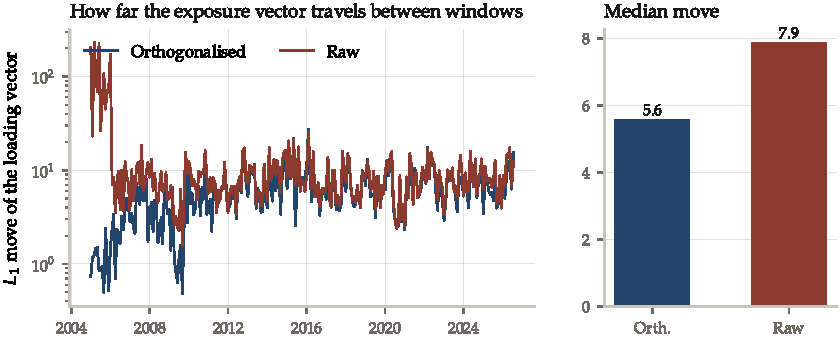
\includegraphics[width=\textwidth]{figures/amzn-stability}
\caption{How far the whole loading vector travels between consecutive windows,
measured in $L_1$ on the factors common to both. Log scale on the left.}
\end{figure}

Aggregated over the whole vector, the raw panel's exposures move a median
\shiftR{} per month against the orthogonalised panel's \shiftO{} --- roughly
\emph{forty per cent further}, every month, for a security whose underlying
business did not change on that schedule. The correlation with the previous window tells the
same story more gently: \corrO{} orthogonalised, \corrR{} raw.

\begin{takeaway}
An exposure estimate that moves this much between windows is not a measurement of
Amazon. It is a measurement of which way the collinearity happened to break in the
last 252 days.
\end{takeaway}

% =====================================================================
\section{Fit: where the raw panel wins}

\begin{figure}[htbp]
\centering
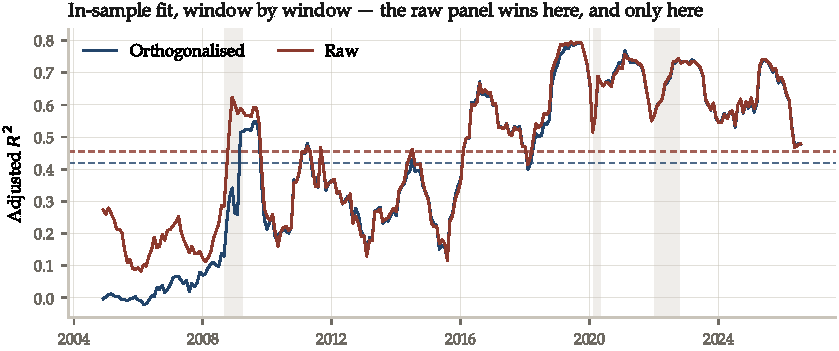
\includegraphics[width=\textwidth]{figures/amzn-fit}
\caption{Adjusted $R^2$ window by window, with each panel's mean as a dashed line.
The raw panel is above the orthogonalised one almost everywhere.}
\end{figure}

Mean adjusted $R^2$ is \adjRR{} on the raw panel against \adjRO{} on the
orthogonalised one, and mean annualised residual volatility is \residR{} against
\residO{}. The raw panel fits better. It is important to say so plainly, because it
is the one statistic an analyst is most likely to look at, and on its own it points
the wrong way.

The reason is mechanical rather than economic. The residualised factors span the
same space as the raw ones up to a rotation, so a perfectly conditioned regression
would give identical fits. The gap is what near-collinearity buys in sample: extra
freedom to fit the particular 252 days in the window, paid for with parameters that
do not generalise.

\begin{figure}[htbp]
\centering
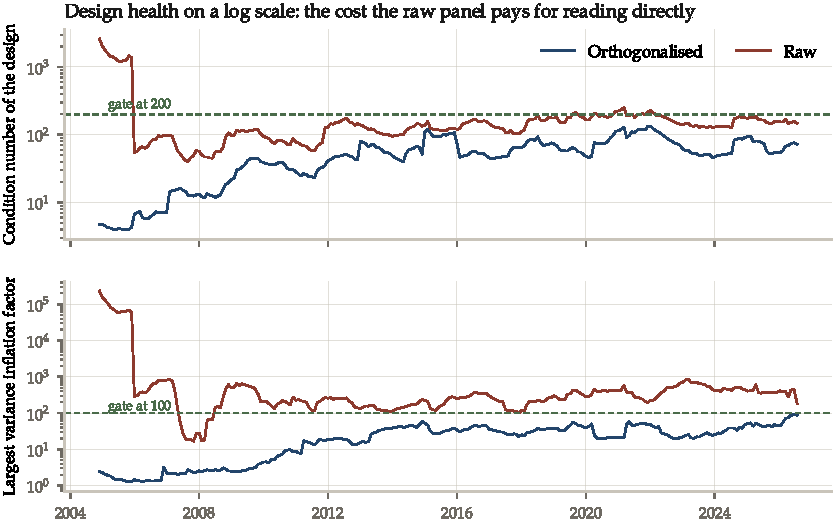
\includegraphics[width=\textwidth]{figures/amzn-conditioning}
\caption{Design health on a log scale. The raw panel's largest variance inflation
factor sits an order of magnitude above the gate for essentially the entire sample
--- which is why the VIF limit is applied only to the orthogonalised panel, and the
condition number to both.}
\end{figure}

The conditioning chart is the same information from the other side. The
orthogonalised design averages a condition number of \condO{} and never exceeds
\condMaxO{}. The raw design averages \condR{} and reaches \condMaxR{}. Its largest
VIF averages \vifR{} and peaks at \vifMaxR{} --- a factor whose $R^2$ against the
other thirty-nine rounds to 0.999996.

\begin{takeaway}
In-sample fit is not evidence about a forecasting model. On this security it is
evidence pointing the wrong way, and the next section is what settles the question.
\end{takeaway}

% =====================================================================
\section{Forecast: where the raw panel loses}

\begin{figure}[htbp]
\centering
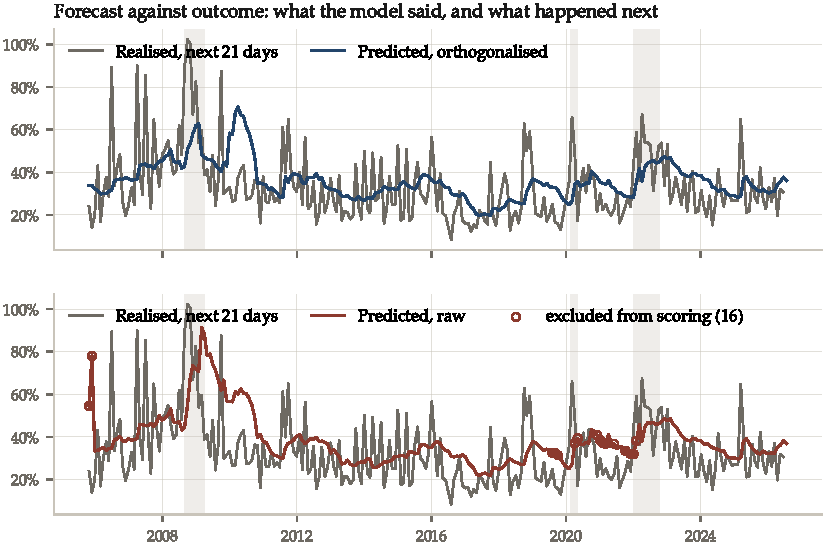
\includegraphics[width=\textwidth]{figures/amzn-forecast}
\caption{Each panel's 21-day volatility forecast against what actually happened
over the following 21 days. Circled points on the lower chart are the \exclR{}
windows the reliability gate excluded from scoring.}
\end{figure}

Both panels track the broad shape of Amazon's volatility. The difference is in how
much of the \emph{variation} each one captures, which is what the Mincer-Zarnowitz
regression measures.

\begin{figure}[htbp]
\centering
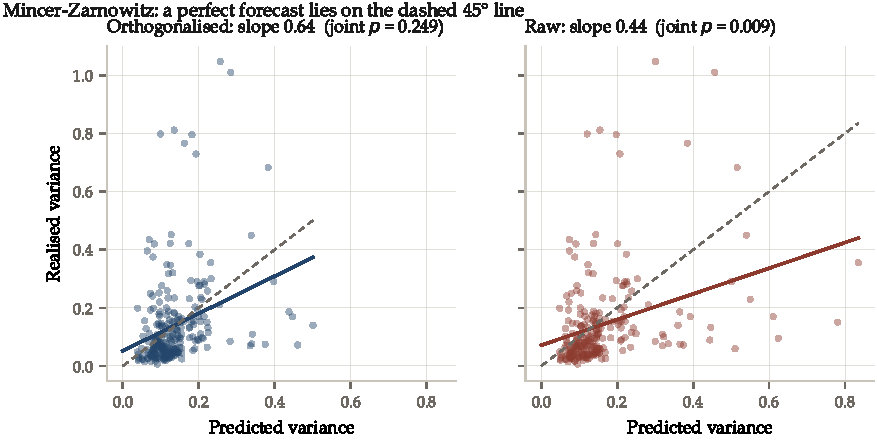
\includegraphics[width=\textwidth]{figures/amzn-mz}
\caption{Realised variance against predicted variance. A perfect forecast lies on
the dashed 45\textdegree{} line; the solid line is the fitted Mincer-Zarnowitz
regression, with HAC standard errors because the forward windows overlap.}
\end{figure}

\begin{center}
\small
\begin{tabular}{@{}lrrl@{}}
\toprule
 & \textcolor{navy}{\textbf{Orthogonalised}} & \textcolor{brick}{\textbf{Raw}} & \textbf{Target} \\
\midrule
Forecasts scored & \nfcO{} & \nfcR{} & --- \\
Windows excluded as ill-conditioned & \exclO{} & \exclR{} & 0 \\
Mean bias ratio & \biasO{} & \biasR{} & 1 \\
Bias statistic (sd of standardised returns) & \zstdO{} & \zstdR{} & 1 \\
Mincer-Zarnowitz slope & \textbf{\mzbO{}} & \mzbR{} & 1 \\
Mincer-Zarnowitz joint $p$ & \textbf{\mzpO{}} & \mzpR{} & $>0.05$ \\
Mincer-Zarnowitz $R^2$ & \mzrO{} & \mzrR{} & high \\
\bottomrule
\end{tabular}
\end{center}

The orthogonalised forecast has a slope of \mzbO{} and is \emph{not} rejected by
the joint test of $(\alpha,\beta) = (0,1)$ at $p$ = \mzpO{}. The raw forecast has a
slope of \mzbR{} and is rejected at $p$ = \mzpR{}. Both get the average level
roughly right --- bias ratios of \biasO{} and \biasR{} --- and the orthogonalised
panel's bias statistic of \zstdO{} is almost exactly the 1 it is aiming at. What
separates them is period-by-period accuracy, and that is the property a risk limit
depends on.

A slope below 1 is partly mechanical at a 21-day horizon, because realised
volatility over a forward window blends regimes while the forecast refers to one;
on simulated data a \emph{perfect} forecast produces a slope near 0.5 when the true
regime length matches the horizon. So \mzbO{} is a respectable number in absolute
terms, and the comparison between \mzbO{} and \mzbR{} is the part that carries no
caveat, because the mechanical effect is identical on both.

\begin{figure}[htbp]
\centering
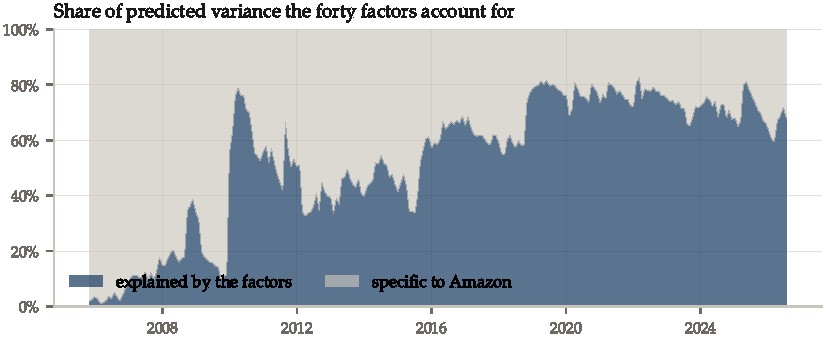
\includegraphics[width=\textwidth]{figures/amzn-risk-share}
\caption{The share of predicted variance the forty factors account for, on the
orthogonalised panel. The remainder is specific to Amazon. The factor share
averages \shareMean{} and exceeds half in \shareMajority{} of windows --- low for
a large-capitalisation equity, and the point of the chart.}
\end{figure}

% =====================================================================
\section{Where the risk sits}

\begin{figure}[htbp]
\centering
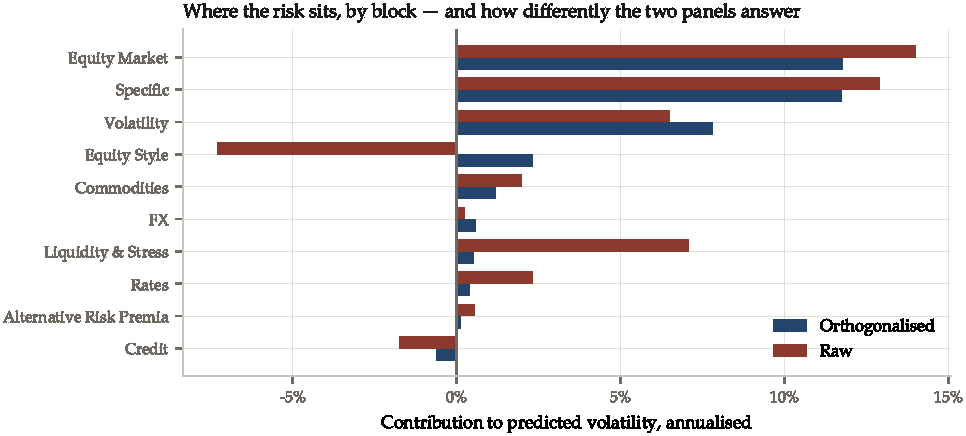
\includegraphics[width=\textwidth]{figures/amzn-blocks}
\caption{Euler risk contributions at \amzWindowEnd{}, aggregated to block, from the
same 504-day blended covariance the forecast used. Contributions sum to the
predicted volatility.}
\end{figure}

At the final window the orthogonalised model predicts \predLastO{} annualised
volatility for Amazon, of which \shareLastO{} of the \emph{variance} is
systematic. In the Euler decomposition --- which splits the volatility rather than
the variance, and so sums exactly to \predLastO{} --- the largest single factor
block is \topBlockO{} at \topBlockShareO{}. An almost equal share, \specShareO{},
is specific: Amazon's own risk, which no factor in the panel explains.

That last number is the honest headline of the whole exercise. Across the whole
sample the forty factors account for an average \shareMean{} of Amazon's predicted
variance, and they exceed half of it in \shareMajority{} of windows. The remainder
is Amazon: its margins, its capital expenditure cycle, its regulatory exposure, its
cloud business. The model does not claim otherwise, and the specific-risk floor
exists so that it cannot.

\begin{takeaway}
The raw panel puts \topBlockShareR{} of predicted volatility in \topBlockR{}
against the orthogonalised panel's \topBlockShareO{} --- and, look at the chart,
assigns \emph{Liquidity \& Stress} several times more risk while giving
\emph{Equity Style} a large negative contribution. Same security, same day, same
covariance method. The blocks disagree because on the raw panel they overlap, so
each is partly crediting the others' exposure.
\end{takeaway}

% =====================================================================
\section{Where both panels fail}

A case study that only reported the comparison it set out to make would be
misrepresenting the model. Both panels fail the value-at-risk tests, and they fail
in the same interesting way.

\begin{figure}[htbp]
\centering
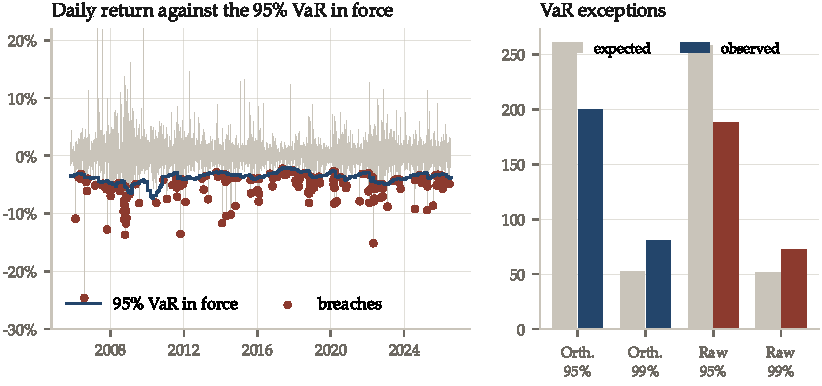
\includegraphics[width=\textwidth]{figures/amzn-var}
\caption{Left: Amazon's daily return against the 95\% value-at-risk in force over
the scored period, on the orthogonalised panel; the VaR steps because the forecast
is refreshed monthly. Right: expected against observed exceptions at both levels
and on both panels.}
\end{figure}

\begin{center}
\small
\begin{tabular}{@{}lrrrr@{}}
\toprule
 & \multicolumn{2}{c}{\textcolor{navy}{\textbf{Orthogonalised}}}
 & \multicolumn{2}{c}{\textcolor{brick}{\textbf{Raw}}} \\
\cmidrule(lr){2-3}\cmidrule(lr){4-5}
 & \textbf{95\%} & \textbf{99\%} & \textbf{95\%} & \textbf{99\%} \\
\midrule
Exceptions expected & \exEFO{} & \exENO{} & \exEFR{} & \exENR{} \\
Exceptions observed & \exNFO{} & \exNNO{} & \exNFR{} & \exNNR{} \\
Kupiec $p$ & \kupFO{} & \kupNO{} & \kupFR{} & \kupNR{} \\
\bottomrule
\end{tabular}
\end{center}

Look at the direction of the miss. At the 95\% level there are \emph{too few}
breaches --- \exNFO{} against \exEFO{} expected. At the 99\% level there are
\emph{too many} --- \exNNO{} against \exENO{}. The model is simultaneously too
cautious in the body of the distribution and too confident in its tail.

That is not a calibration error in the volatility forecast, which the bias
statistic of \zstdO{} says is very nearly right. It is the Gaussian quantile
assumption failing. After dividing every return by the volatility forecast that was
current on that day, the standardised series still has an excess kurtosis of
\zkurtO{} --- barely reduced from the raw \amzKurt{}. Scaling the distribution
correctly does not make it normal, and Amazon's is emphatically not.

\begin{takeaway}
Both panels also fail the Christoffersen conditional-coverage test, with $p$-values below 0.001: the breaches cluster. That
is expected when a 21-day-horizon forecast is applied to daily returns, it is the
same on both panels, and it is therefore not evidence about the panel choice --- but
it is a limit of the forecast and is reported as one.
\end{takeaway}

The practical consequence is narrow and worth stating: use this model's volatility
forecast, and treat its Gaussian VaR as a lower bound on the tail. The Student-$t$
quantile the risk module also offers is the better default for a security like this
one.

% =====================================================================
\section{Verdict}

\begin{center}
\small
\begin{tabularx}{\textwidth}{@{}lX@{}}
\toprule
\textbf{Question} & \textbf{Answer for Amazon} \\
\midrule
How much equity risk? & Raw panel. Read \code{eq\_global} + \code{eq\_us} as a
single total exposure; the split between them is not identified. \\
What explains the returns? & Orthogonalised panel. Global beta, a cyclical tilt,
a negative momentum loading --- each incremental over the blocks above it. \\
How risky is it next month? & Orthogonalised panel, \predLastO{} annualised.
The raw panel's forecast is rejected by the joint Mincer-Zarnowitz test. \\
Where does the risk come from? & Orthogonalised panel. \specShareO{} of predicted
volatility is specific to Amazon and no factor in the panel explains it. \\
How bad can a day get? & Neither, on a Gaussian quantile. The standardised
returns still have excess kurtosis of \zkurtO{}. \\
\bottomrule
\end{tabularx}
\end{center}

The general finding this case study supports is the one the model is built around:
the in-sample statistic and the out-of-sample statistic disagree, and the
out-of-sample one is right. On a single security, with every other setting held
fixed, the raw panel bought \adjRR{}$-$\adjRO{} of adjusted $R^2$ and paid for it
with a Mincer-Zarnowitz slope of \mzbR{} instead of \mzbO{}, \exclR{} unusable
windows instead of \exclO{}, and a loading vector that travels
forty per cent further every month.

\vspace{1.2ex}
{\footnotesize\color{ink}
Reproduce with:\\[0.4ex]
\code{python -m backend.pipeline.sync --security US:AMZN}\\
\code{python -m backend.pipeline.run\_estimation --instrument US:AMZN --window 252 --step 1m}\\
\code{python -m backend.pipeline.run\_estimation --instrument US:AMZN --window 252 --step 1m --raw-factors}\\
\code{python -m backend.pipeline.run\_risk --instrument US:AMZN --spec \orthSpec\ldots{} --horizon 21}\\
\code{python -m scripts.build\_case\_study --pdf}\\[0.6ex]
Every figure and every number above is generated by the last command from the
database; none is typed by hand.\par}

\end{document}
